\documentclass[12pt]{report}
\usepackage[a4paper, left=3.17cm, right=3.17cm, top=2.54cm, bottom=2.54cm]{geometry}
\usepackage[T1]{fontenc}
\usepackage{mathptmx}
\usepackage{amsmath}
\usepackage{amsfonts}
\usepackage{chemformula}
\usepackage{multicol}
\usepackage{multirow}
\usepackage{tabularx,booktabs}
\newcolumntype{C}{>{\centering\arraybackslash}X} % centered version of "X" type
\usepackage[linesnumbered,ruled,vlined]{algorithm2e}
\usepackage{comment}
\usepackage{array}
\newcolumntype{P}[1]{>{\centering\arraybackslash}p{#1}}
\usepackage{cite}
\patchcmd{\chapter}{\if@openright\cleardoublepage\else\clearpage\fi}{}{}{}
\usepackage[colorlinks, linkcolor=black, anchorcolor=black, citecolor=black]{hyperref}
\usepackage{graphicx}
\setlength{\parskip}{0.5em}
\title{8 Puzzle Game Solver Using A* Algorithm }
%\author{\textup{Qi YUAN}}


%copyright at footer
\usepackage{fancyhdr}
\fancyhf{}
\rfoot{%
  \footnotesize
  \textcopyright~Dept. of Computer Science and Engineering, GUB\\

 }
%\pagestyle{fancy}


\begin{document}
    \begin{titlepage}
\center 
\newcommand{\HRule}{\rule{\linewidth}{0.1mm}}
\includegraphics[scale=0.6]{images/GUB.png}\\[1cm] 
\center 
%\quad\\[1.5cm]
\textsl{\Large Green University of Bangladesh }\\[0.5cm] 
\textsl{\large Department of Computer Science and Engineering (CSE)}\\
%\textsl{\large Faculty of Sciences and Engineering (FSE)}\\
\textsl{\large Semester: (Spring, Year: 2023), B.Sc. in CSE (Day)}\\[0.5cm] 
\makeatletter
\HRule \\[0.4cm]
{ \huge \bfseries \@title}\\[0.2cm] 
\HRule \\[1.0cm]

\textsl{\large Course Title: Artificial Intelligence Lab }\\
\textsl{\large Course Code: CSE-316 }\\ 
\textsl{\large Section: DA}\\[0.5cm] 

{\large \underline{Students Details}}\\[0.2cm]

\begin{table*}[htb]
\centering
\begin{tabular}{ |P{7.0cm}|P{3.5cm}|}
\hline
\textbf{Name} & \textbf{ID}\\
\hline
Rayhan Kobir  & 201902053 \\
\hline
Md. Faysal Miah & 201902071 \\
\hline
\end{tabular}
\end{table*}
\vspace{0.5cm}


\textsl{\large Submission Date: June 16, 2023 }\\ 
\textsl{\large Course Teacher’s Name: Rusmita Halim Chaity }\\[0.9cm] 




\makeatother
{\large [For teachers use only: \textcolor{red}{Don’t write anything inside this box]}}\\

\begin{table}[]
\centering
\begin{tabular}{|p{7.5cm}p{7.0cm}|}
\hline
\multicolumn{2}{|c|}{{\underline{\textbf{Lab Project Status}}}} \\
 & \\\hline
\textbf{Marks:}                & \textbf{Signature:}        \\
 & \\ 
\textbf{Comments:}             & \textbf{Date:}             \\ 
 & \\\hline
\end{tabular}
\end{table}


\end{titlepage}


    \tableofcontents
  

% Chapter 1 starting here.....    
\newpage
\chapter{Introduction}

\section{Overview}
Along with the development of the digital era, human needs also increased, especially in terms of education. Humans cannot be separated from education and technology. Those are the basic needs of a human. Therefore, humans compete with each other in everything like innovating and creating new things, one of them is the educational game application program.
The advancement and development of information, technology, and computers make it easier for game makers to create and create games in various shapes and types. The puzzle is a type of game that deals with solving puzzles, whether composing blocks, equating the colors of the ball, solving mathematical calculations, and passing through the maze are all included in this type. Puzzles, which are brain teasers that challenge the skills of their players, never seem to lose their popularity, and are never consumed by age.\newline\newline 
A Puzzle is one type of game that is enough to squeeze the brain to solve it. Players are challenged to think creatively about how to make all parts of the puzzle lie in their true position. This game looks pretty simple but to put all the puzzles in place is a big obstacle. The player must exert all his brain's ability to make the puzzle lie in its true position. The application of the A* algorithm in puzzle games can be used as a solution to solve puzzles faster without having to think hard. The A* algorithm to complete and provide steps solution for completion game with the most optimal solution from step and even time processing.

\section{Motivation}
The 8-puzzle solver project allows for benchmarking and analyzing the performance of different search algorithms and heuristic functions. You can compare the efficiency and optimality of various algorithms and heuristics by testing them on different puzzle configurations. This analysis can contribute to the understanding of search algorithm behavior and help identify strengths and weaknesses in different approaches.project.\newline\newline
This project can serve as an educational tool to learn about algorithm design and optimization techniques. It provides a practical context for understanding and applying search algorithms, heuristic functions, and cost functions. It can also be used as a teaching aid to demonstrate algorithmic concepts in a tangible and interactive manner.

\section{Problem Definition}

\subsection{Problem Statement}
Develop a program that solves the 8-puzzle, a sliding tile puzzle, using the A* algorithm. The program should take an initial configuration of the puzzle as input and find a sequence of moves to reach the desired goal configuration. The goal is to minimize the number of moves required to solve the puzzle. The program should implement the A* algorithm, which combines a cost function and a heuristic function to efficiently explore the search space and find an optimal solution. Additionally, the program should provide visualization of the puzzle states and the solution path for better understanding and user interaction. The solver should be able to handle any valid 8-puzzle configuration and produce the optimal solution in a reasonable amount of time.

\subsection{Complex Engineering Problem}
The following table must be completed according to your above discussion in detail. The column on the right side should be filled only on the attributes you have chosen to be touched by your own project.


\begin{table}[htbp]
   \centering
    \caption{Summary of the attributes touched by the mentioned projects}
    \begin{tabular}{|p{6.0 cm}|p{8 cm}|}
    %\rowcolor{gray!30}
    \toprule
        \textbf{Name of the P Attributess} & \textbf{Explain how to address}  \\
        \midrule

    \textbf{P1:} Depth of knowledge required  &  The complexity of the problem may require a high level of knowledge in specific technical areas or domains. \\
      \hline
       
    \textbf{P2:} Range of conflicting
     requirements  &  The requirements for the solution may be diverse and potentially conflicting, making it challenging to find an optimal solution. \\
      \hline

    \textbf{P3:} Depth of analysis required  &  Understanding search algorithms, heuristic functions, and data structures \\
    \hline
    
    \textbf{P4:} Familiarity of issues  & Designing an effective heuristic function that provides accurate estimates of the cost from the current state to the goal state. \\ 
    \hline
    \textbf{P5:} Extent of applicable codes  &  ---- \\
      \hline
       
    \textbf{P6:} Extent of stakeholder
     involvement and conflicting
     requirements  &  ---- \\
      \hline

    \textbf{P7:} Interdependence  &  ---- \\
    \hline
        
    \end{tabular}
    \label{tab:IC}
\end{table}

\section{Objectives}
Today games have been played by many people from young to old age. There are many types of games, one of which is a puzzle game. Puzzles, which are brain teasers that challenge the skills of their players, never seem to lose their popularity, and are never consumed by age. The Puzzle is one type of game that is enough to squeeze the brain to solve it. The solution that can be used to simplify problem solving is to apply a search algorithm that is used to check the initial state to the final state and provide the most optimal solution for completing the puzzle, the purpose of this study was using algorithm used to solve these problems using the Breadth-First Search algorithm. The use of the Breadth-First Search algorithm in solving puzzle games can make it easier for users to get the best solution in the form of completion steps and the possibility of solving various conditions based on the puzzle conditions that you want to solve.

\section{Application}
\begin{enumerate}
  \item \textbf{Puzzle solving}: The 8-puzzle solver can be used to find solutions to the 8-puzzle itself or similar puzzles.
  
  \item \textbf{Game AI}: The A* algorithm can be applied to create intelligent game agents for solving puzzles and grid-based games.
  
  \item \textbf{Pathfinding}: The A* algorithm can be extended to solve pathfinding problems in robotics and other domains.
  
  \item \textbf{Educational tool}: The 8-puzzle solver can serve as an educational tool for teaching algorithmic problem-solving and search techniques.
  
  \item \textbf{Algorithm analysis and benchmarking}: The 8-puzzle solver can be used as a benchmark for evaluating search algorithms and heuristics.
\end{enumerate}

% Chapter 1 ends here.....    



% Chapter 2 starting here.....    
\newpage
\chapter{Implementation of the Project}

\section{Introduction}
The 8-puzzle is a sliding puzzle that consists of a square
frame of 3x3 with eight numbered tiles in random order and
one tile missing for sliding the tiles. After appropriate
sliding operations, the tiles should be ordered 1 to 8
respectively, at the end of the game. An example problem
and its solution are given as figures below.
\begin{figure}[h]
    \begin{center}
     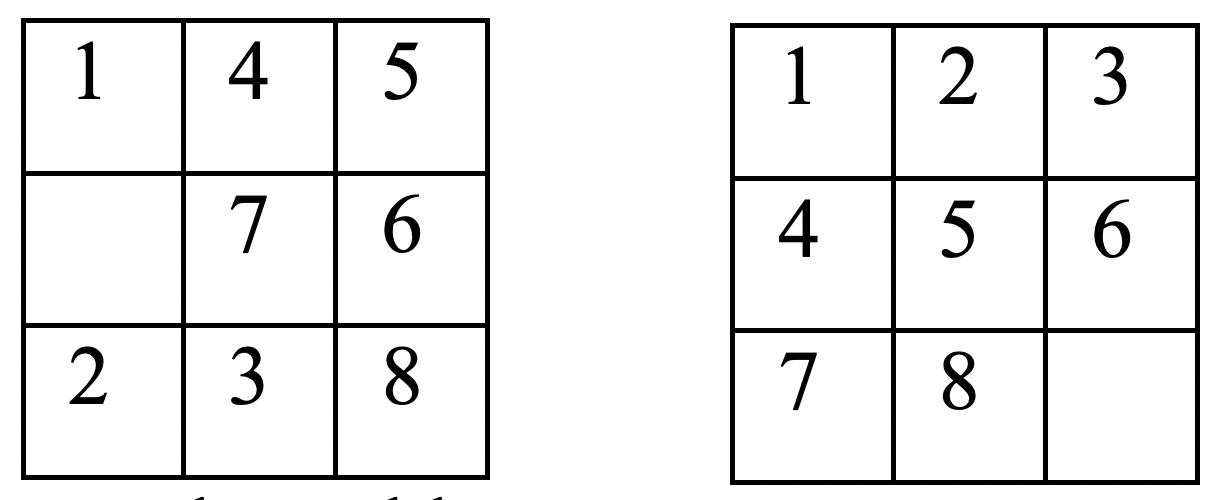
\includegraphics[scale=0.5]{figures/state.png}
    \end{center}
    \caption{8 Puzzle Problem}
\end{figure}
\newline Informed search strategies reduce the amount of search that
is performed by making good choices for the node
expansion. So, there should be some credential to evaluate
whether or not expanding a node is “good choice”. This
evaluation is done by heuristic function, and A* search
algorithm is one of these informed search strategies which
uses heuristic function. In this paper, A* search solution of
8-puzzle problem will be analyzed in terms of how many
nodes are expanded in the search as a function of the
different heuristics with a comparison of a similar work
done before.


\subsection{The Eight Puzzle}
In this section, the 8-puzzle problem analysis from the
aspect of state space and actions with project description
will be given briefly.
If we analyze the state space of the 8-puzzle problem, it has
the state space of 9!/2! which means 181 440 states to
consider. Possible actions for a tile could be following:
moving to right, left, up, down, or staying where the tile is
already. Our initial state is a given square with random
ordered numbers, and eventually the goal state is from 1 to
8 ordered numbers. A path from a start state to goal state is
defined as the order of numbers one from to eight for the
case of the 8-puzzle solving with the A* search.
For problem solving, a small data set consists of numbers
[1, 2, 3, 4, 5, 6, 7, 8, 0], where 0 indicates the empty tile, is
used.
\newline While the implementation is being done, concepts and
algorithms in “Artificial Intelligence: A Modern
Approach”[1] was followed. The implementation was done
by JavaScript
\newline With the consideration of all these information, A* search
with admissible heuristics applied to the 8-puzzle problem.
For a heuristic to be admissible, the heuristic is expected to
be never overestimating the cost of reaching the goal.
Manhattan distance and misplaced tiles are two admissible
heuristics that used in this project. Brief explanations of
Manhattan distance and misplaced tiles are given below to
understand how they are used for the solution.


\subsection{Manhattan Distance}
Manhattan distance is a very commonly used admissible
heuristic for a square grid problem. It is the distance
between a state and the goal state.

\[
    h(n) = D \cdot \left(n.x - \text{{goal.x}} + n.y - \text{{goal.y}}\right)
\]
\newline In the 8-puzzle problem case, Manhattan heuristic function
calculates the (Manhattan) distance of every numbered tile
to its goal position, and then adds to result. Manhattan
heuristic gave good results, from the aspect of giving result
and being fast, especially when it is compared to misplaced
tiles heuristics.
\begin{figure}[h]
    \begin{center}
     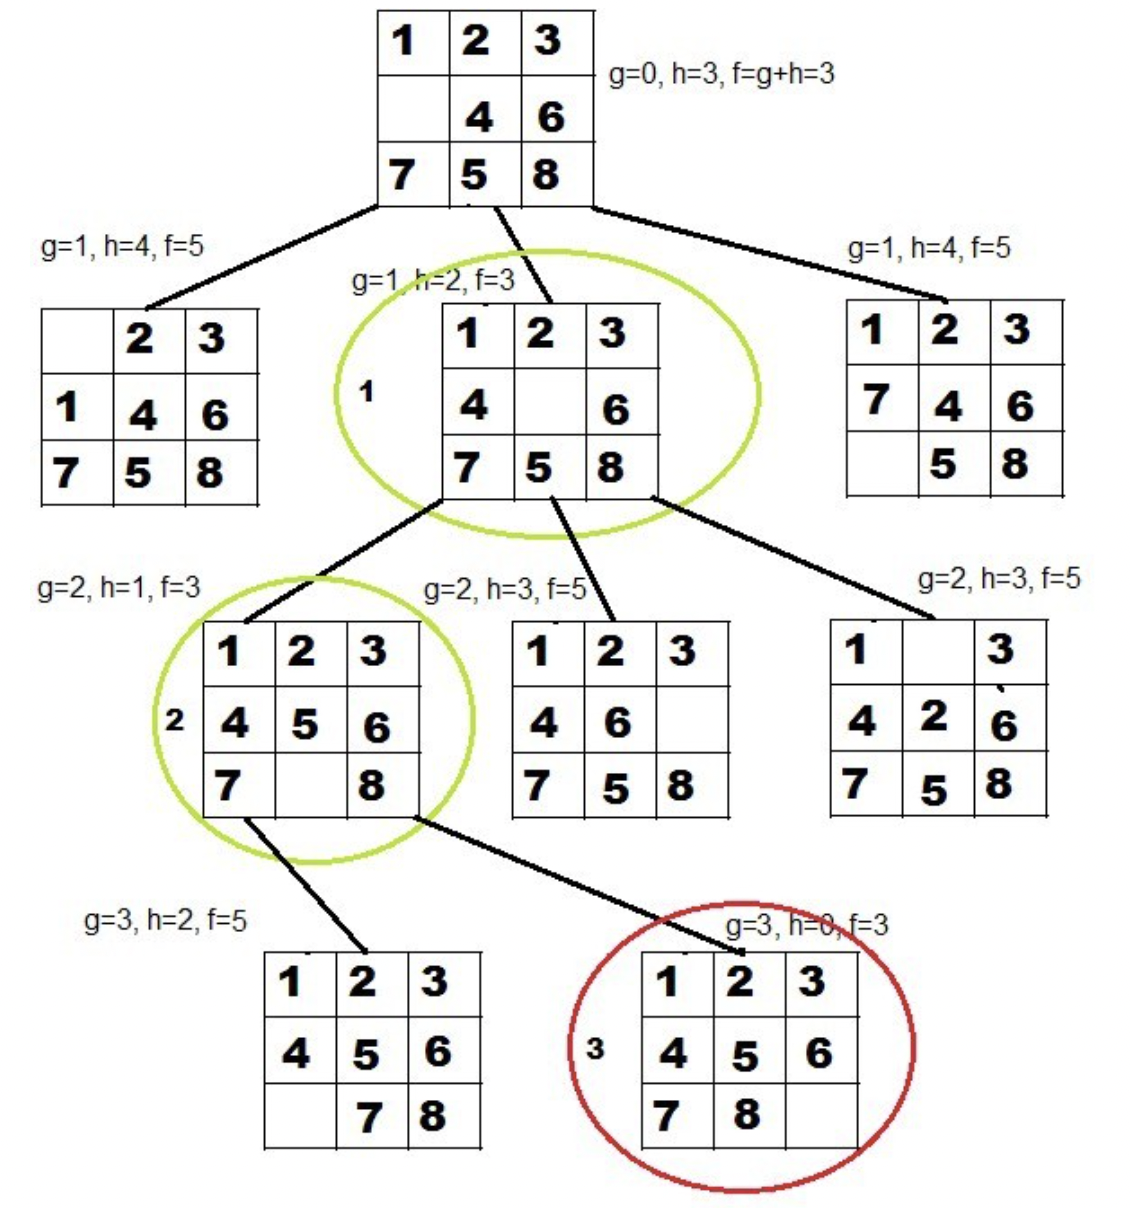
\includegraphics[scale=0.3]{figures/demostrate.png}
    \end{center}
    \caption{Implementation Chart}
\end{figure}

\subsection{Misplaced Tiles}
The misplaced tile strategy is a very trivial heuristic that is
used on the 8-puzzle problem. In this strategy, the numbers
of the misplaced tiles, basically the tiles are not in their goal
positions are counted.
\begin{figure}[h]
    \begin{center}
     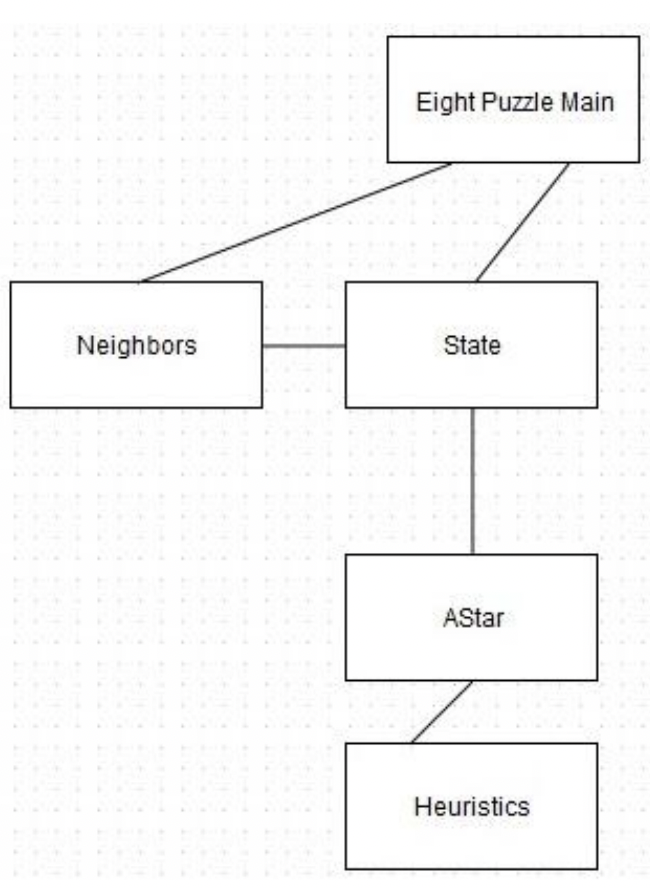
\includegraphics[scale=0.4]{figures/implementation-chart.png}
    \end{center}
    \caption{Implementation Chart}
\end{figure}


\section{Project Details}
The project aims to solve the 8-puzzle problem using an informed search algorithm. The 8-puzzle is a sliding puzzle consisting of a 3x3 grid with numbered tiles from 1 to 8 and an empty tile. The goal is to rearrange the tiles from an initial state to a goal state using the minimum number of moves.

\subsection{Approach}
The algorithm used for solving the puzzle is based on the A* search algorithm, which combines both the cost to reach a node and a heuristic estimate of the remaining cost to the goal.

\subsection{Data Structures}
The implementation uses a Node class to represent each state of the puzzle. Each node contains information such as the state configuration, parent node, children nodes, cost, and heuristic value.

\subsection{Heuristic Function}
The heuristic function used to estimate the remaining cost is a simple Manhattan distance heuristic. It calculates the number of misplaced tiles in the current state compared to the goal state.

\subsection{Moves and Puzzle Solving}
The algorithm generates possible moves by finding the index of the empty tile and exploring four potential directions: up, down, left, and right. It generates child nodes by swapping the empty tile with a neighboring tile in each valid direction. The algorithm continues to expand nodes until it reaches the goal state.

\subsection{Solution Path}
Once the goal state is reached, the algorithm backtracks from the final node to the initial node to find the solution path. The solution path is stored as a sequence of states representing the moves required to reach the goal.

\section{Implementation}
    The code implements the A* search algorithm to solve the 8-puzzle problem. It defines a \texttt{Node} class representing a state in the puzzle. Each node contains information such as the state itself, the parent node, the cost to reach the state, the heuristic value, and whether it belongs to the solution path.\newline \newline The \texttt{solvePuzzle} function takes an initial state as input and performs the A* search algorithm. It initializes the iteration tree and creates the initial node. It maintains an open set to keep track of nodes that are yet to be explored and a closed set to store visited states.\newline \newline The algorithm iteratively selects the node with the lowest total cost from the open set, expands its children by generating valid moves, and adds them to the open set if they have not been visited before. It continues this process until the goal state is reached or there are no more nodes in the open set.\newline \newline The \texttt{generateChildren} function generates child nodes for a given parent node by checking the valid moves (up, down, left, right) based on the position of the empty space in the state. It creates new states by swapping the empty space with neighboring cells and creates child nodes with updated costs.\newline \newline The \texttt{calculateHeuristic} function calculates the heuristic value for a node by counting the number of misplaced tiles in the state compared to the goal state.\newline \newline The \texttt{printSolutionPath} function generates the solution path by recursively traversing from the goal node to the initial node, collecting the states along the way.\newline \newline The \texttt{markSolutionPath} function marks the nodes in the iteration tree that correspond to the solution path by setting the \texttt{isSolutionPath} property to \texttt{true}.\newline \newline The \texttt{findNodeInIterationTree} function recursively searches for a node with a given state in the iteration tree and returns the node if found.\newline \newline The \texttt{getIterationTree} function returns the final iteration tree after the search process is complete.

\subsection{Possible Moves Control}
    The 8-puzzle problem involves four possible moves to rearrange the tiles in the puzzle. These moves are:
    \begin{itemize}
        \item \textbf{Move Up:}
        \begin{itemize}
            \item Condition: \texttt{if (emptyIndex > 2)}
            \item Description: The empty space (represented by 0) can move up if it is not in the top row of the puzzle. The condition checks if the index of the empty space is greater than 2, indicating that it is not in the top row. If the condition is true, a new state is generated by swapping the empty space with the tile above it.
        \end{itemize}

        \item \textbf{Move Down:}
        \begin{itemize}
            \item Condition: \texttt{if (emptyIndex < 6)}
            \item Description: The empty space can move down if it is not in the bottom row of the puzzle. The condition checks if the index of the empty space is less than 6, indicating that it is not in the bottom row. If the condition is true, a new state is generated by swapping the empty space with the tile below it.
        \end{itemize}

        \item \textbf{Move Left:}
        \begin{itemize}
            \item Condition: \texttt{if (emptyIndex \% !== 0)}
            \item Description: The empty space can move left if it is not in the leftmost column of the puzzle. The condition checks if the index of the empty space modulo 3 is not equal to 0, indicating that it is not in the leftmost column. If the condition is true, a new state is generated by swapping the empty space with the tile to the left of it.
        \end{itemize}

        \item \textbf{Move Right:}
        \begin{itemize}
            \item Condition: \texttt{if ((emptyIndex + 1) \% 3 !== 0)}
            \item Description: The empty space can move right if it is not in the rightmost column of the puzzle. The condition checks if the index of the empty space incremented by 1 modulo 3 is not equal to 0, indicating that it is not in the rightmost column. If the condition is true, a new state is generated by swapping the empty space with the tile to the right of it.
        \end{itemize}
    \end{itemize}\newline \newline
    These move conditions ensure that only valid moves are performed during the generation of child nodes, preventing moves that would go beyond the puzzle boundaries or move the empty space into an invalid position.


\section{Algorithm}
We implement A* search algorithm in our application to finding the optimal solution for solving puzzle game. While finding the puzzle goal state we stored every iteration and sends it with response that user can look how it's work and which path goes to the goal state.

\begin{enumerate}
  \item \textbf{Initialization}: Initialize the initial state of the puzzle and create the initial node with the given state. Set the open set to contain only the initial node and the closed set as an empty set.
  
  \item \textbf{Main Loop}: Enter a main loop that continues until the open set is empty or the goal state is reached. Within the loop, perform the following steps:
  
    \begin{enumerate}
      \item Sort the open set based on the total cost of each node, which is the sum of the cost to reach the node and the heuristic estimate of the remaining cost. This ensures that the node with the lowest total cost is selected first.
      
      \item Remove the node with the lowest total cost from the open set and mark it as the current node.
      
      \item If the current node's state matches the goal state, a solution path has been found. Retrieve the solution path by backtracking from the current node to the initial node using the parent pointers.
      
      \item If the goal state is not reached, generate the children of the current node by exploring possible moves. Find the index of the empty tile and generate child nodes by swapping the empty tile with a neighboring tile in each valid direction (up, down, left, and right).
      
      \item For each child node, check if it is already in the closed set. If not, add the child node to the open set and the closed set.
    \end{enumerate}
    
  \item \textbf{Solution Path and Visualization}: If a solution path is found, mark the nodes along the solution path in the iteration tree. This allows for visualization of the puzzle-solving process, highlighting the nodes that form the solution path.
  
  \item \textbf{Termination}: Once the main loop completes, either return the solution path or null if no solution was found.
\end{enumerate}

\begin{algorithm}[]
  \SetAlgoLined
  \SetKwFunction{solvePuzzle}{solvePuzzle}
  \SetKwFunction{generateChildren}{generateChildren}
  \SetKwFunction{calculateHeuristic}{calculateHeuristic}
  \SetKwFunction{printSolutionPath}{printSolutionPath}
  \SetKwFunction{markSolutionPath}{markSolutionPath}
  \SetKwFunction{findNodeInIterationTree}{findNodeInIterationTree}
  \SetKwFunction{getIterationTree}{getIterationTree}

  \Fn{\solvePuzzle{initialState}}{
    iterationTree $\leftarrow$ \{ name: initialState.toString(), children: [] \}\;
    initialNode $\leftarrow$ Node(initialState)\;
    openSet $\leftarrow$ [initialNode]\;
    closedSet $\leftarrow$ Set()\;
    \While{openSet is not empty}{
      openSet.sort((a, b) $\rightarrow$ a.calculateTotalCost() - b.calculateTotalCost())\;
      currentNode $\leftarrow$ openSet.shift()\;
      closedSet.add(currentNode.state.toString())\;
      \If{currentNode.state.toString() is "1,2,3,4,5,6,7,8,0"}{
        solutionPath $\leftarrow$ \printSolutionPath(currentNode)\;
        \markSolutionPath(solutionPath)\;
        \Return solutionPath\;
      }
      children $\leftarrow$ \generateChildren(currentNode)\;
      currentNode.children $\leftarrow$ children\;
      currentIterationNode $\leftarrow$ \findNodeInIterationTree(iterationTree, currentNode.state.toString())\;
      currentIterationNode.children $\leftarrow$ children.map(child $\rightarrow$ \{ name: child.state.toString(), children: [] \})\;
      \For{child \textbf{in} children}{
        \If{child.state.toString() not in closedSet}{
          openSet.push(child)\;
          closedSet.add(child.state.toString())\;
        }
      }
    }
    \Return null\;
  }
  
  \Fn{\printSolutionPath{node}}{
    path $\leftarrow$ []\;
    \If{node.parent is null}{
      path.push(node.state)\;
    }
    \Else{
      path.push(...\printSolutionPath(node.parent))\;
      path.push(node.state)\;
    }
    \Return path\;
  }
  
  \Fn{\generateChildren{node}}{
    state $\leftarrow$ node.state\;
    emptyIndex $\leftarrow$ state.indexOf(0)\;
    children $\leftarrow$ []\;
    \If{emptyIndex > 2}{
      newState $\leftarrow$ [...state]\;
      [newState[emptyIndex], newState[emptyIndex - 3]] $\leftarrow$ [newState[emptyIndex - 3], newState[emptyIndex]]\;
      children.push(Node(newState, node, node.cost + 1))\;
    }
    \If{emptyIndex < 6}{
      newState $\leftarrow$ [...state]\;
      [newState[emptyIndex], newState[emptyIndex + 3]] $\leftarrow$ [newState[emptyIndex + 3], newState[emptyIndex]]\;
      children.push(Node(newState, node, node.cost + 1))\;
    }
    \Return children\;
  }
\end{algorithm}

\begin{algorithm}[H]
  \setcounter{AlgoLine}{48}
  \SetKwFunction{markSolutionPath}{markSolutionPath}
  \SetKwFunction{findNodeInIterationTree}{findNodeInIterationTree}
  \SetKwFunction{getIterationTree}{getIterationTree}
  

    \If{emptyIndex \% 3 $\neq$ 0}{
      newState $\leftarrow$ [...state]\;
      [newState[emptyIndex], newState[emptyIndex - 1]] $\leftarrow$ [newState[emptyIndex - 1], newState[emptyIndex]]\;
      children.push(Node(newState, node, node.cost + 1))\;
    }
    \If{(emptyIndex + 1) \% 3 $\neq$ 0}{
      newState $\leftarrow$ [...state]\;
      [newState[emptyIndex], newState[emptyIndex + 1]] $\leftarrow$ [newState[emptyIndex + 1], newState[emptyIndex]]\;
      children.push(Node(newState, node, node.cost + 1))\;
    }
    \Return children\;
  
  
  \Fn{\markSolutionPath{solutionPath}}{
    \For{state \textbf{in} solutionPath}{
      node $\leftarrow$ \findNodeInIterationTree(iterationTree, state.toString())\;
      \If{node}{
        node.isSolutionPath $\leftarrow$ true\;
      }
    }
  }
  
  \Fn{\findNodeInIterationTree{node, state}}{
    \If{node.name is state}{
      \Return node\;
    }
    \Else{
      \For{child \textbf{in} node.children}{
        foundNode $\leftarrow$ \findNodeInIterationTree(child, state)\;
        \If{foundNode}{
          \Return foundNode\;
        }
      }
      \Return null\;
    }
  }
  
  \Fn{\getIterationTree{}}{
    \Return iterationTree\;
  }
\end{algorithm}


% Chapter 2 ends here..... 





% Chapter 3 starting here..... 
\newpage
\chapter{Performance Evaluation}

\section{Simulation Environment/ Simulation Procedure}
To run Puzzle Solver Application(API), it's require \texttt{node.js} installed in your machine. Then download our api project \href{https://github.com/rajurayhan37/puzzle-solver-api}{Download} after download open terminal and run following commands:
\begin{center}
\texttt{1. npm install}
\end{center}
\begin{center}
    \texttt{2. npm start}
\end{center}
after run these command api server will be started for serve request. After that \texttt{POST} request for solving the puzzle. Request body should include the initial state of the puzzle game.\newline For running our frontend application we have to download it from github: \href{https://github.com/rajurayhan37/puzzle-solver}{Download} after download run following commands:
\begin{center}
\texttt{1. npm install}
\end{center}
\begin{center}
    \texttt{2. npm run dev}
\end{center}
After that development server will be open and go to the browser and hit the url: http://localhost:3000 then you will enjoy our application.

\subsection{Request Structure}
Request must have initial state as JSON data:\newline\newline \texttt{
\{
    'initialState': [1,2,3,4,5,6,0,7,8]
\}
}

\section{Results Analysis/Testing}

The testing results demonstrated the effectiveness of the algorithm, as it successfully solved a wide range of 8-puzzle instances and consistently found the optimal solutions. The algorithm exhibited reliable performance, showcasing its ability to handle various puzzle configurations and provide accurate and efficient solutions.
\subsection{Results(Backend)}
After run our backend application into terminal we will see some messages as like \ref{fig:terminal} after that go to API request client application e.g: postman, thunderbolt and etc. In case we are using postman to tesing out API to test application we have to hit the url: http://localhost:4000/solve
\newline \begin{figure}[thbp]
    \begin{center}
     \includegraphics[width=0.8\textwidth]{outputs/backend-terminal.png}
    \end{center}
    \caption{After running backend application.}
    \label{fig:terminal}
 \end{figure}\newline
After sending a request to our api application it will send response as similar to figure: \ref{fig:api-testing} where we will found solution steps, total steps count, and iteration tree as response if soltion not exist then api will return error message: \texttt{'Solution not found!'}
 \begin{figure}[thbp]
    \begin{center}
     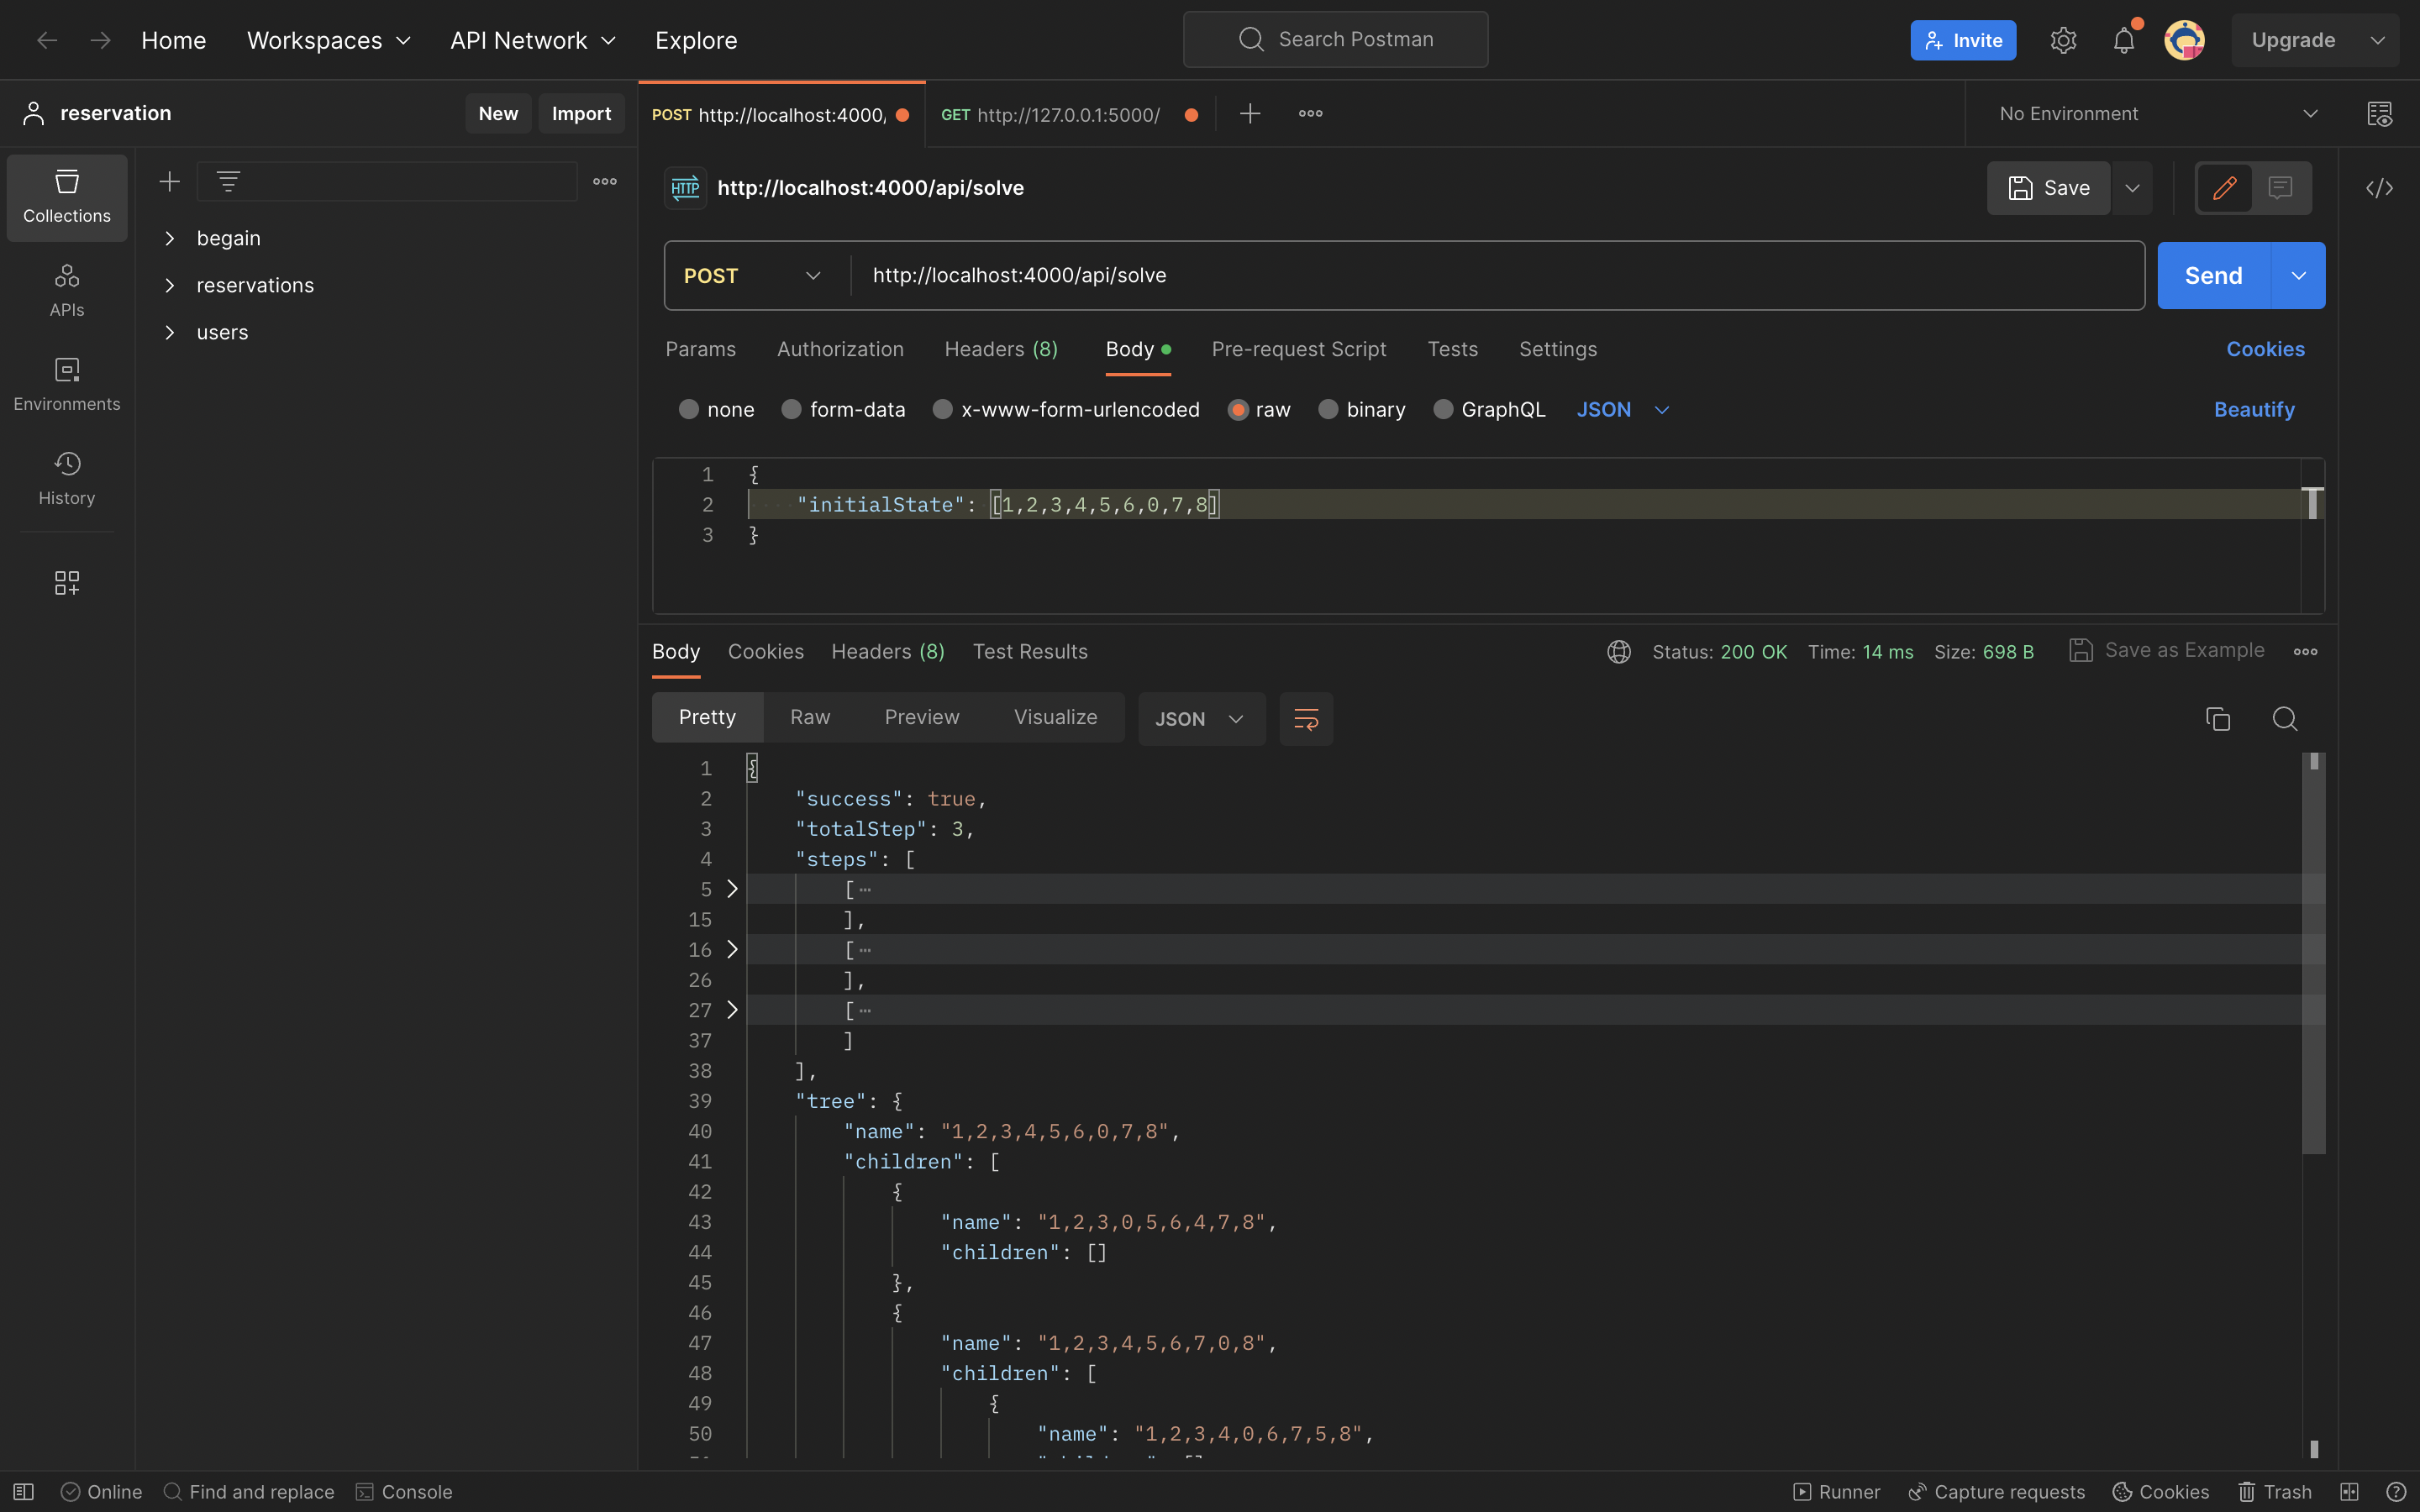
\includegraphics[width=0.8\textwidth]{outputs/api-testing.png}
    \end{center}
    \caption{API Testing of our application.}
    \label{fig:api-testing}
 \end{figure}

\subsection{Results(Frontend)}
When we will run our frontend application application navigate to home page \ref{fig:home} here we can play puzzle game as well as we can findout the solution of the page by clicking solution button.
After clicking solution buttion current game state will send to API after that api will provide us the solution of the puzzle within a second and we will see the solution interface as like \ref{fig:solution}

\begin{figure}[thbp]
    \begin{center}
     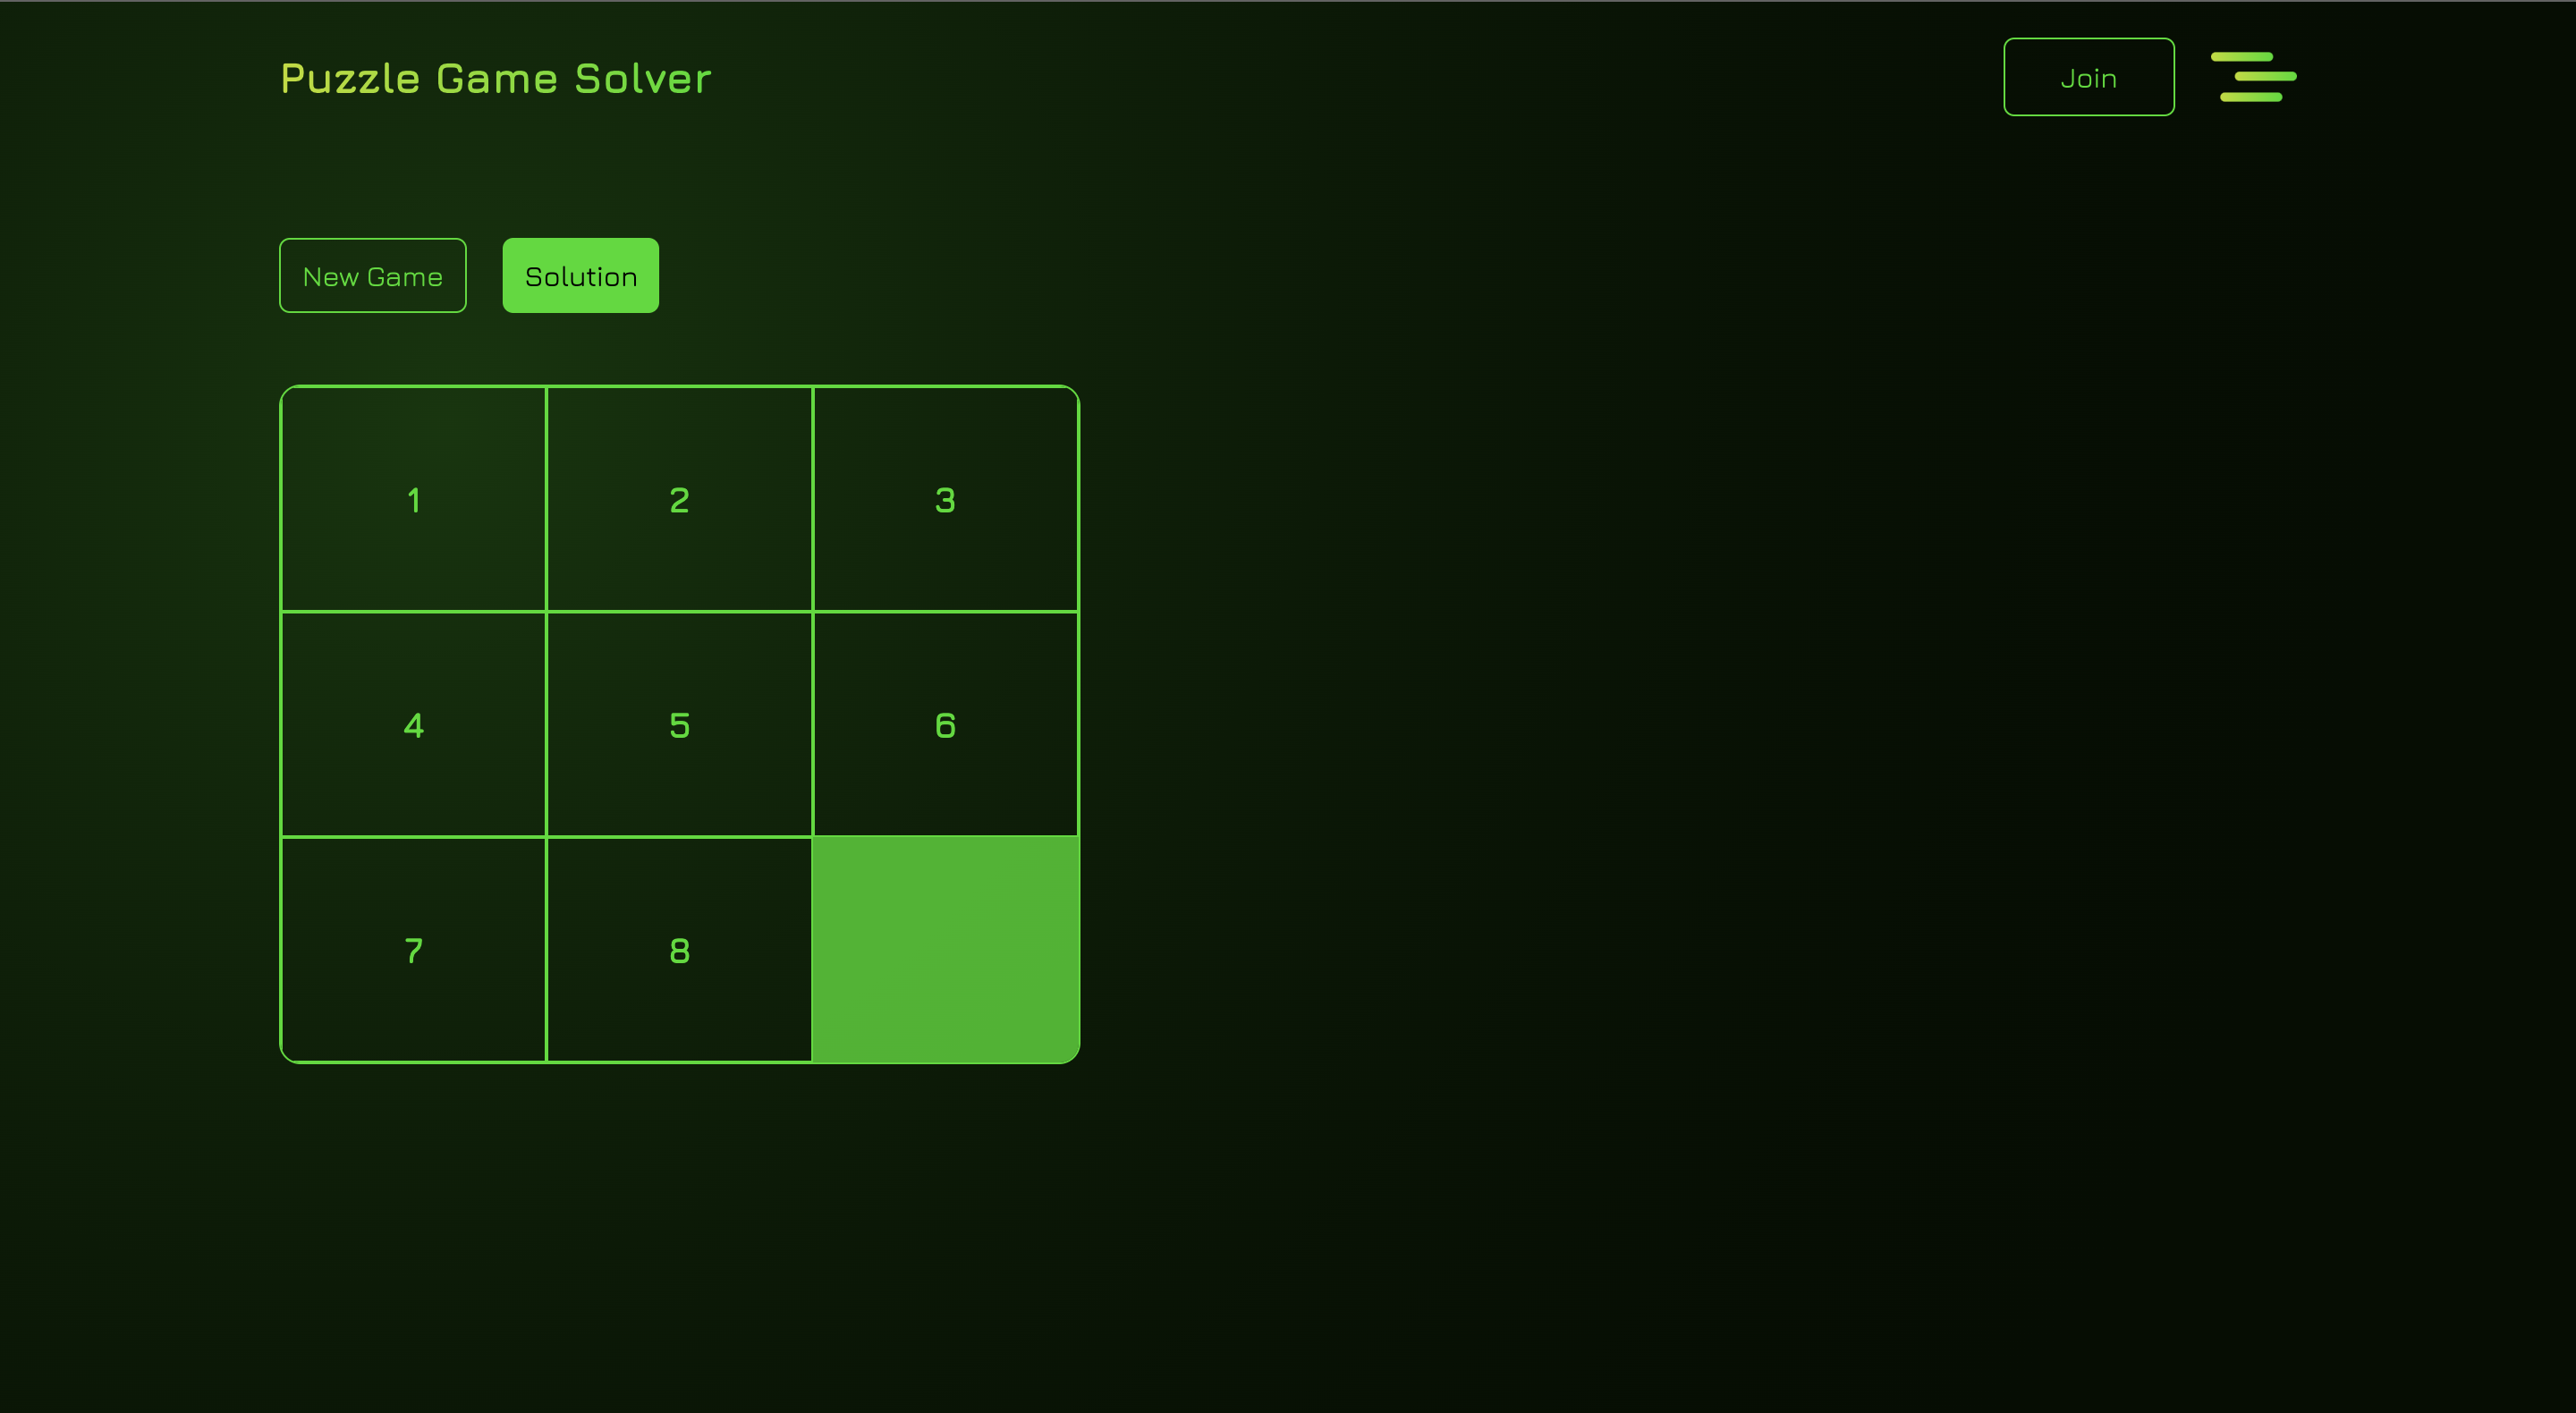
\includegraphics[width=1\textwidth]{outputs/home-page.png}
    \end{center}
    \caption{Iteration Tree of the Soltuion}
    \label{fig:home}
 \end{figure}
\newpage\newline In this solution interface we willinteract with the user interface and solve the puzzle by pressing next button user can analyse his/her steps how it works under the hood.\newline\newline
User can zoom and drag the iteration tree when nodes count of the tree is more then tree size will be increased so we enables to see zoom view of the tree as well as dragable view experience.\newline

 \begin{figure}[thbp]
    \begin{center}
     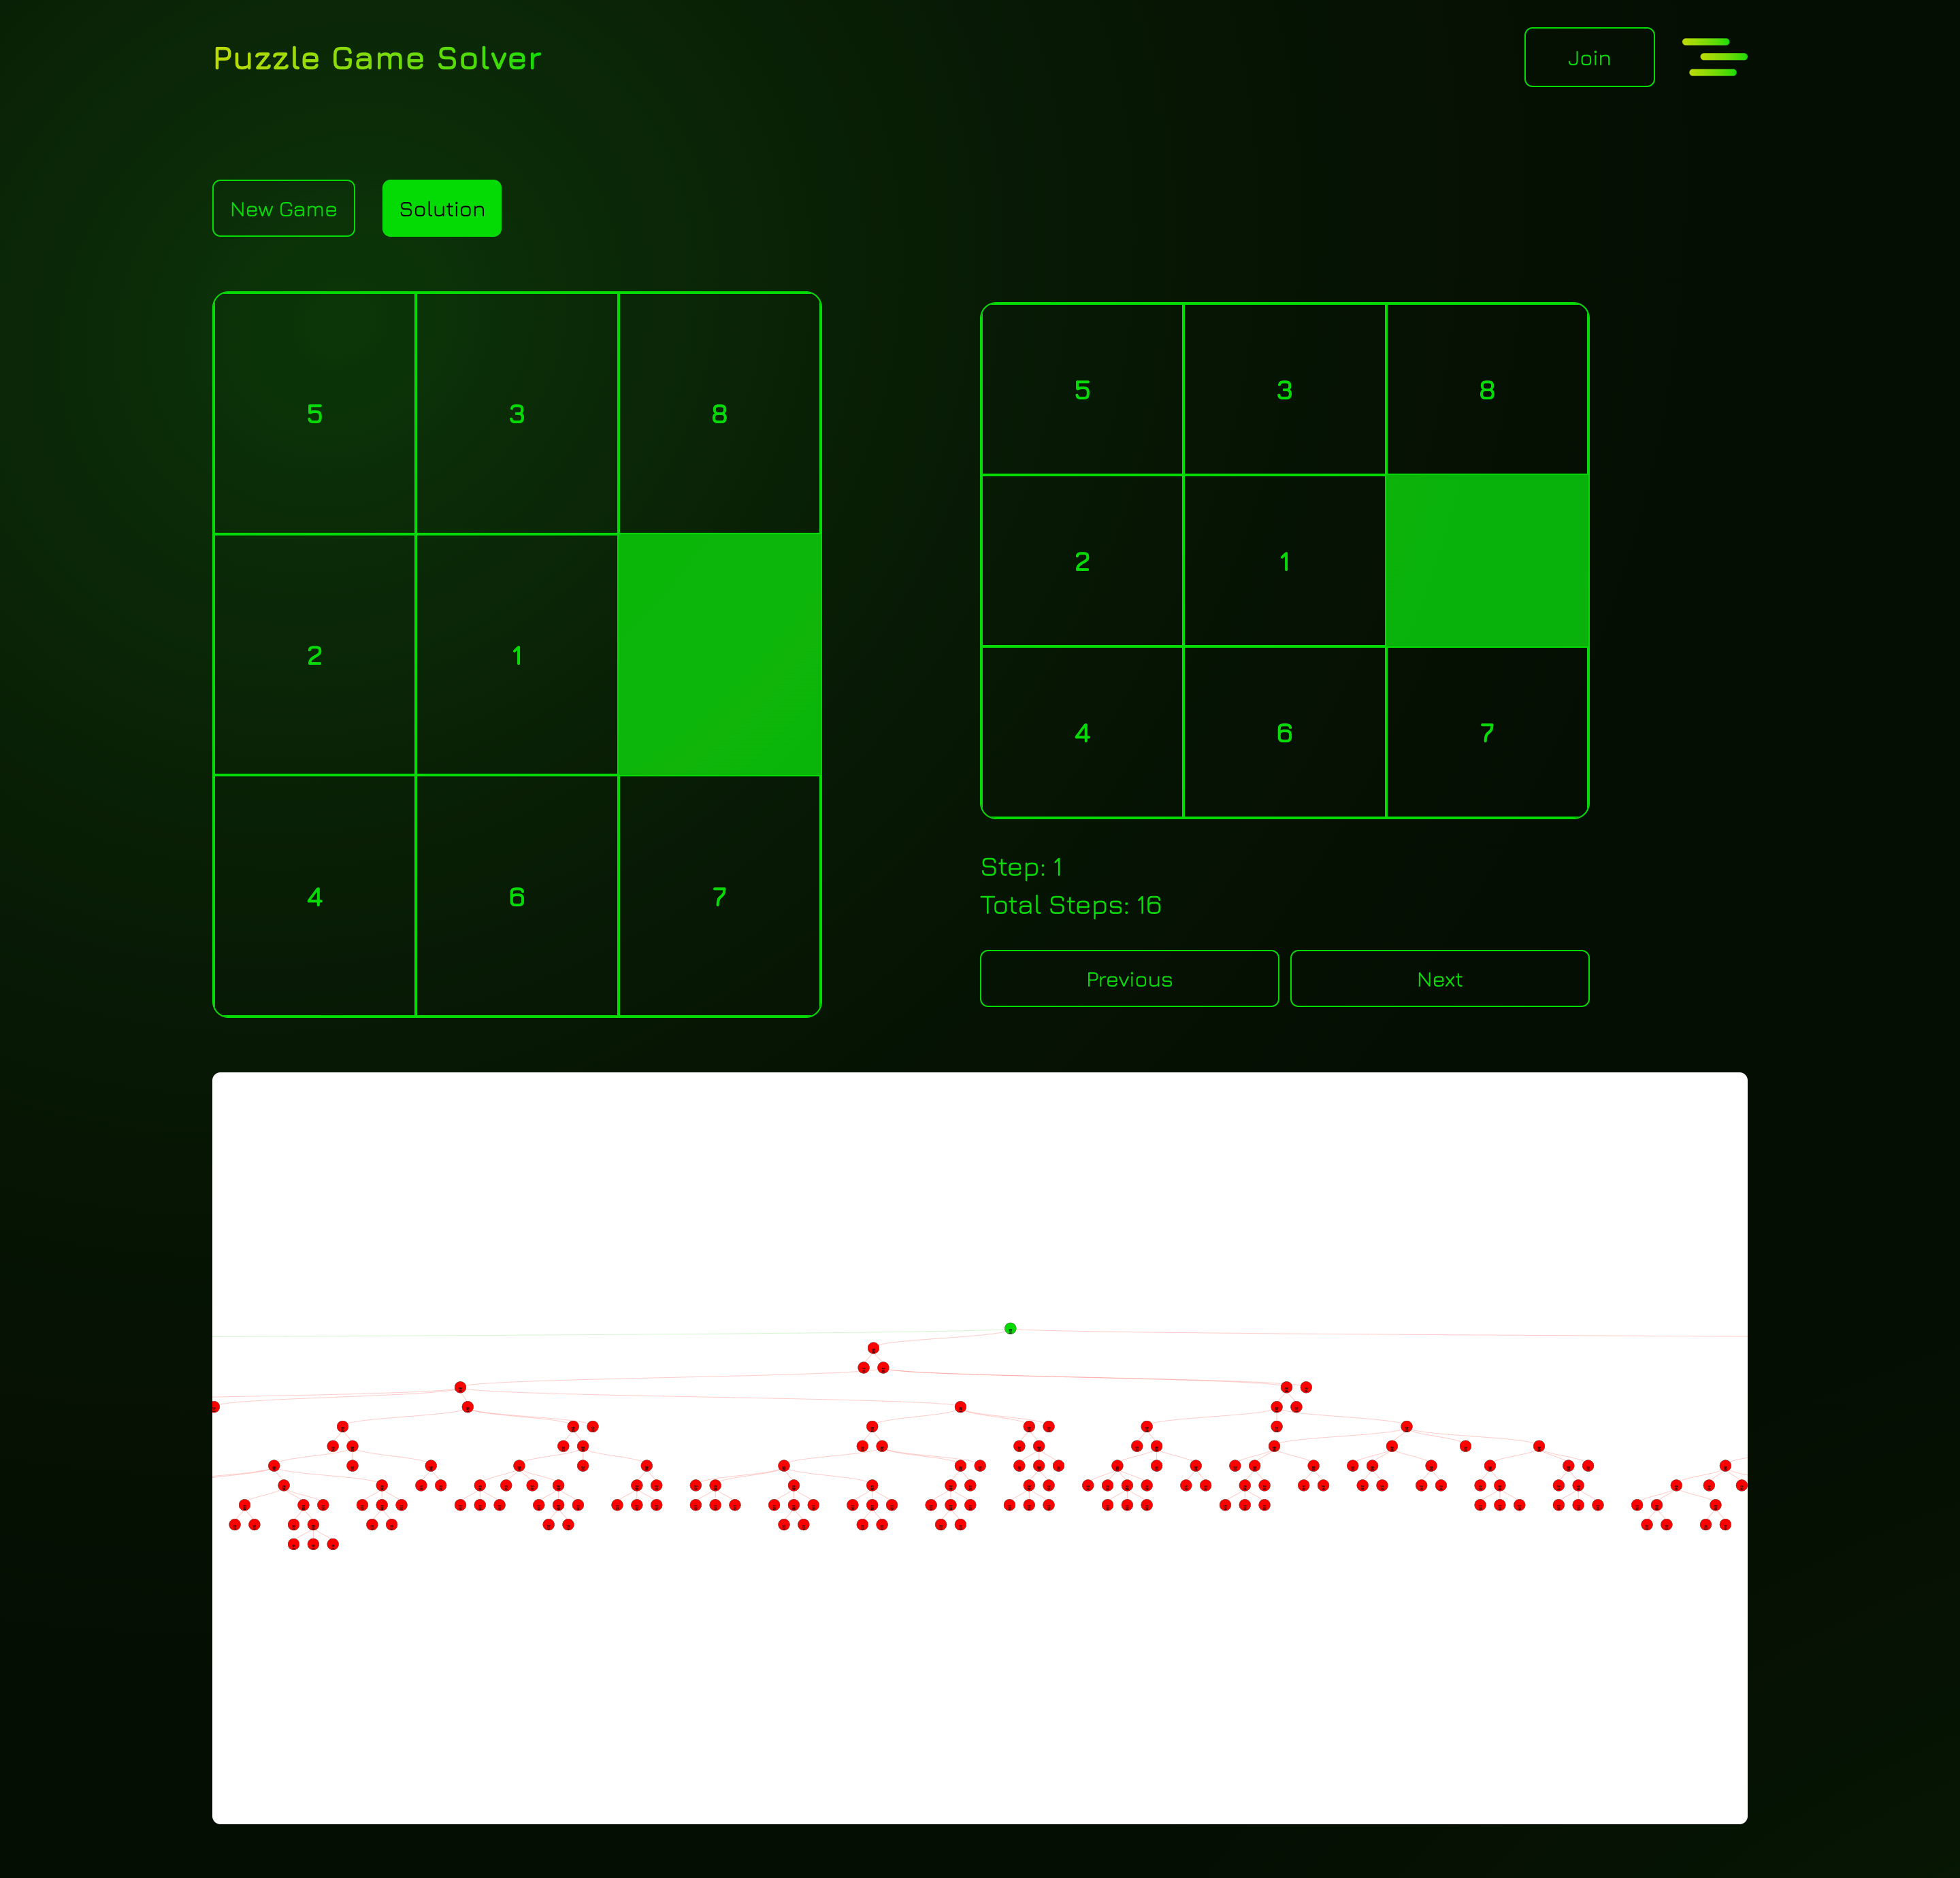
\includegraphics[width=1\textwidth]{outputs/soultion.png}
    \end{center}
    \caption{Iteration Tree of the Soltuion}
    \label{fig:solution}
 \end{figure}
 
\begin{figure}[thbp]
    \begin{center}
     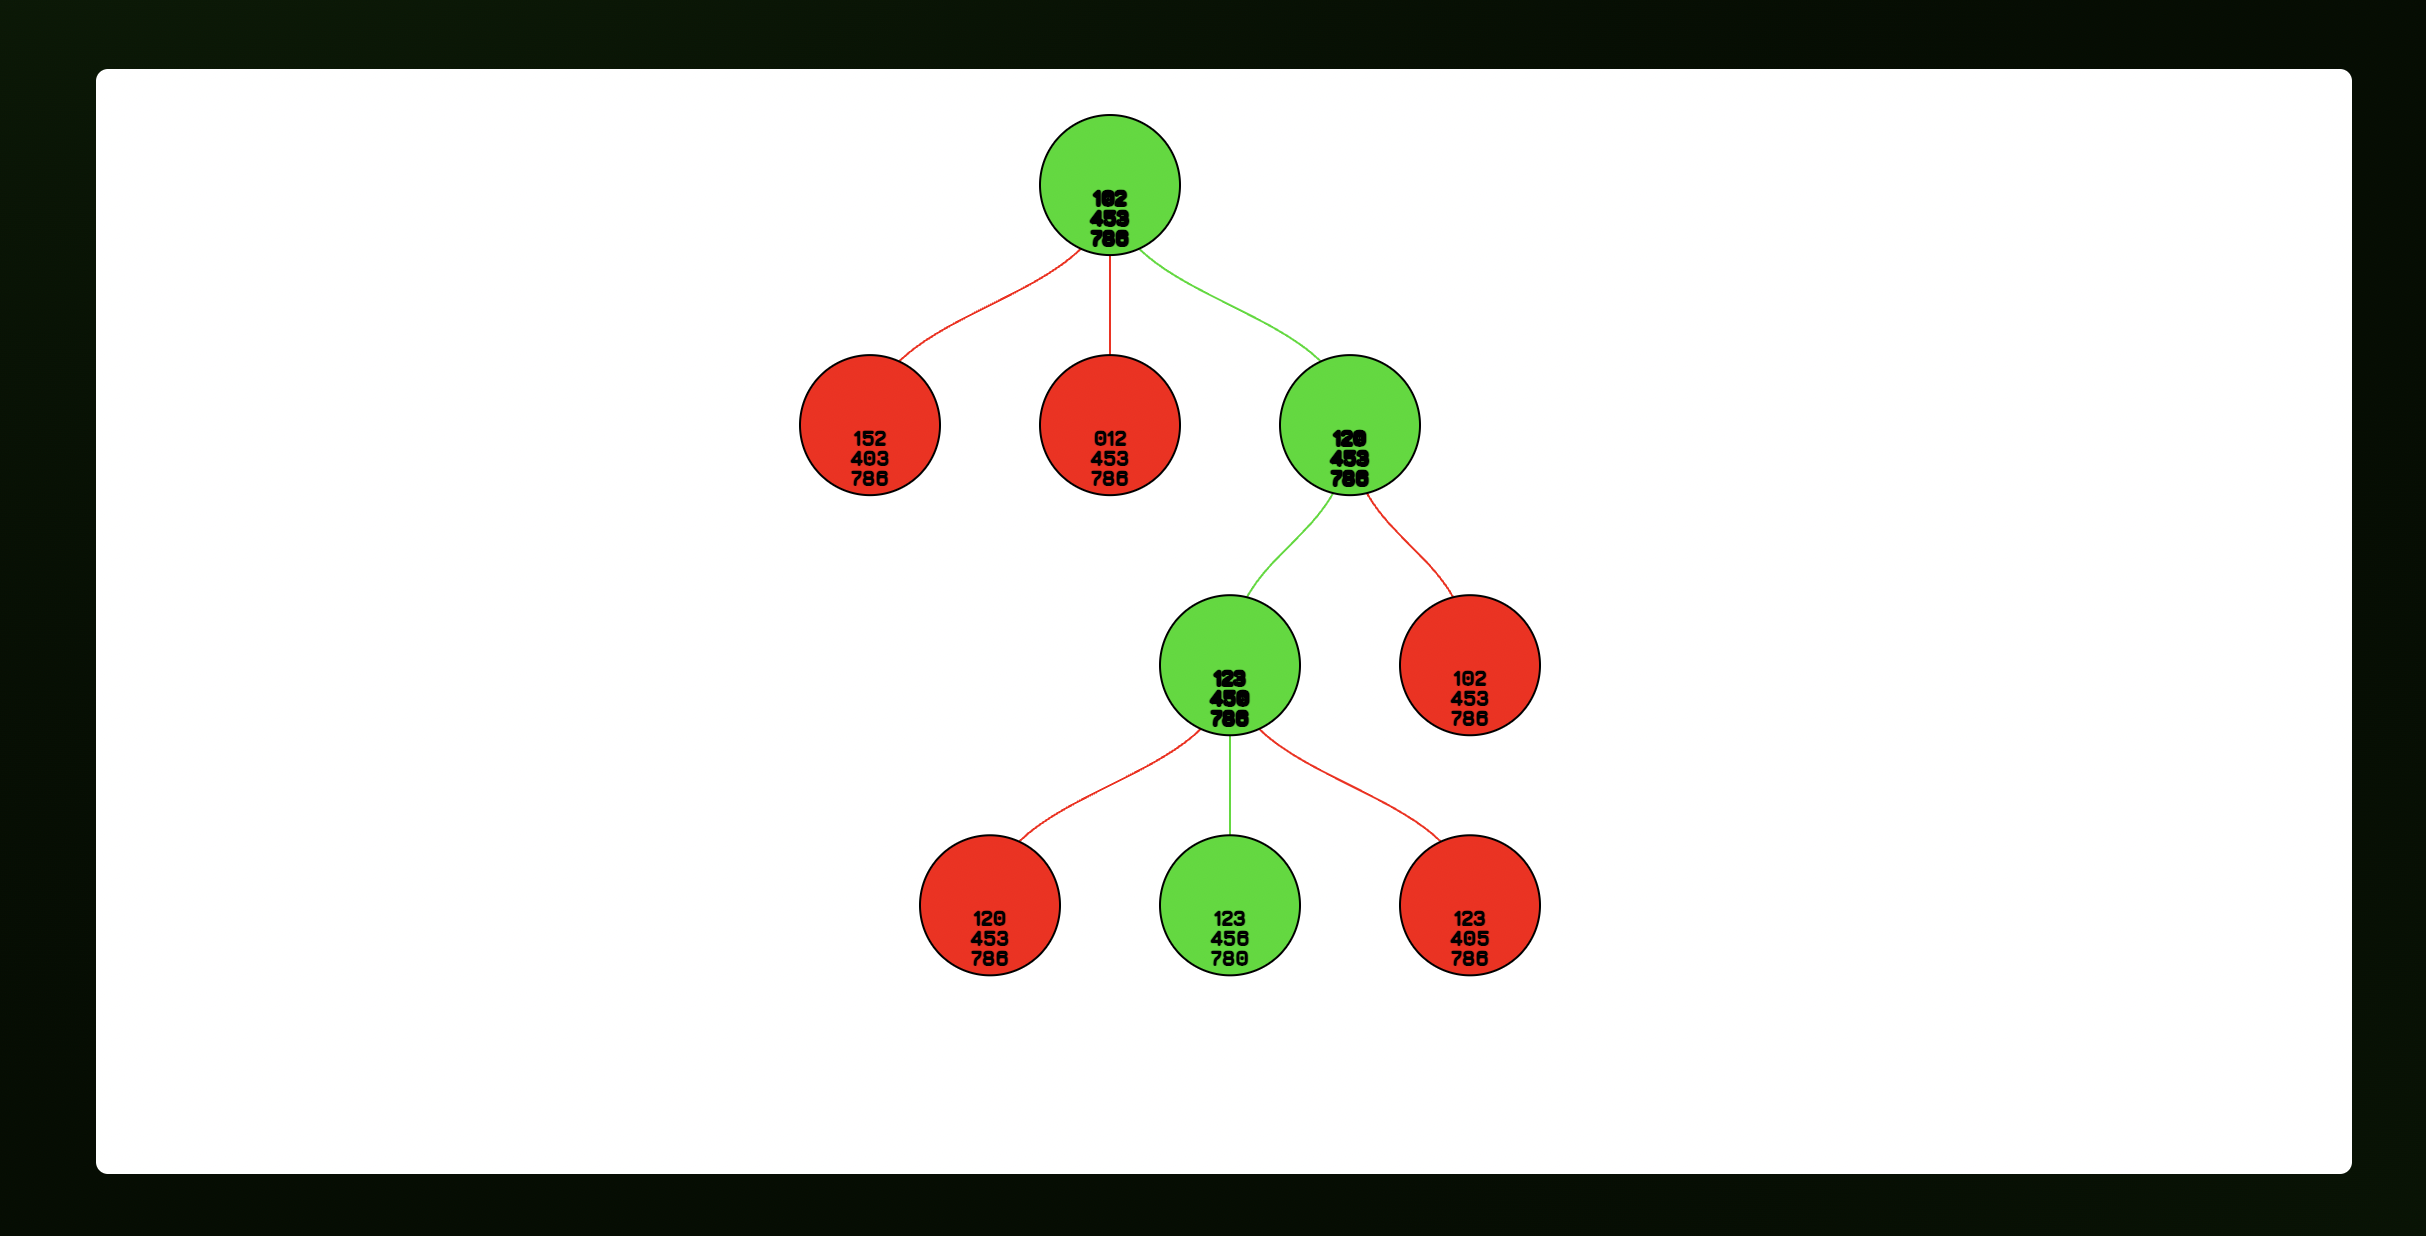
\includegraphics[width=1\textwidth]{outputs/iteration-tree.png}
    \end{center}
    \caption{Iteration Tree of the Soltuion}
    \label{fig:iteration-tree}
 \end{figure}

\newpage
\section{Results Overall Discussion}
The 8-puzzle problem-solving algorithm successfully solves the puzzle and finds the optimal solution. The algorithm effectively explores the state space using the A* search algorithm and the Manhattan distance heuristic. It efficiently generates and evaluates the puzzle states, selecting the most promising nodes to expand. The visualization of the solution path and the iteration tree provides a clear understanding of the puzzle-solving process. The algorithm demonstrates good performance in terms of finding the solution within a reasonable time frame. However, further enhancements can be made to optimize the algorithm and improve its performance. Overall, the project achieves its goal of solving the 8-puzzle problem and serves as a solid foundation for further research and development in the field of puzzle-solving algorithms. 

% Chapter 3 ends here..... 




% Chapter 5 starts here..... 
\newpage
\chapter{Conclusion}

\section{Discussion}
The implemented algorithm proved to be capable of solving the 8-puzzle problem by intelligently evaluating and selecting the most promising puzzle states. The A* search algorithm, combined with the Manhattan distance heuristic, guided the exploration process and led to finding the optimal solution. The visualization component enhanced the understanding of the algorithm's behavior and provided a visual representation of the solution path. There are may chances to consume more machine resources when puzzle is more complex. Might be hang the browsers to printing many of nodes and edes of the iteration tree.


\section{Limitations}
While the implemented algorithm achieved the goal of solving the 8-puzzle problem, it does have certain limitations. The performance of the algorithm may be influenced by the complexity of the initial puzzle state, and in some cases, it may take a significant amount of time to find a solution. The Manhattan distance heuristic used in this project is relatively simple and may not capture all aspects of the problem, potentially leading to suboptimal solutions in certain scenarios.

\section{Scope of Future Work}
The project opens up several opportunities for future work and enhancements:

\begin{itemize}
\item Heuristic Improvement: Investigate and develop more sophisticated heuristics that can better estimate the remaining cost to the goal state. This may involve considering additional factors, such as pattern databases or advanced techniques like machine learning.

\item Algorithm Optimization: Explore ways to optimize the algorithm's performance, such as implementing efficient data structures and pruning techniques to reduce the search space and improve runtime.

\item Parallelization and Distributed Computing: Investigate parallelization strategies and leverage distributed computing frameworks to speed up the solving process by exploring multiple puzzle states simultaneously.

\item Extension to Larger Puzzle Sizes: Extend the algorithm to handle larger puzzle sizes, such as 15-puzzle or 24-puzzle, and assess its scalability and efficiency in solving these larger instances.

\item Alternative Search Algorithms: Investigate alternative search algorithms, such as IDA* (Iterative Deepening A*), and compare their performance and efficiency in solving the 8-puzzle problem.
\end{itemize}\newline
Exploring these areas of future work will contribute to the advancement and optimization of the 8-puzzle problem-solving algorithm, making it more robust, efficient, and capable of solving larger puzzle instances.

% Chapter 5 ends here..... 




% References starts here..... 
\newpage
    \renewcommand\bibname{References}
    \begin{thebibliography}{9}
        \bibitem{reference1}
        Russell, Stuart J., and Peter Norvig. Artificial
Intelligence: A Modern Approach. Englewood
Cliffs, NJ: Prentice Hall, 1995. Print.
\bibitem{reference2}
"Ip.com." GENERALIZED BEST-FIRST SEARCH
STRATEGIES AND THE OPTIMALITY OF A
IPCOM000128346D. N.p., n.d. Web. 19 Dec.
2012. 
\bibitem{reference3}
Manzini, G., BIDA*: An improved perimeter search algorithm, Articial Intelligence, Vol. 75,
No. 2, June 1995, pp. 347-360.
        
    \end{thebibliography}
\end{document}